\documentclass[20pt,a4paper]{extarticle}
\usepackage[utf8]{inputenc}
\usepackage[english]{babel}

\usepackage{amsmath}
\usepackage{amsfonts}
\usepackage{amssymb}
\usepackage{mathtools}
\usepackage{systeme}
\sysdelim..

\usepackage{graphicx}
\usepackage{caption}
\usepackage{subcaption}
\usepackage{lmodern}
\usepackage{tikz}
\usetikzlibrary{calc}
\usepackage{titlesec}
\usepackage{environ}
\usepackage{xcolor}
\usepackage{fancyhdr}
\usepackage[colorlinks = true, linkcolor = black]{hyperref}
\usepackage{xparse}
\usepackage{enumitem}
\usepackage{comment}
\usepackage{wrapfig}
\usepackage{soul}
\usepackage[capitalise]{cleveref}

\usepackage[left=2cm,right=2cm,top=1cm,bottom=3cm]{geometry}
\usepackage{multicol}
\usepackage[indent=0pt]{parskip}

\newcommand{\spaceP}{\vspace*{0.5cm}}
\newcommand{\Span}{\mathrm{Span}\,}
\newcommand{\range}{\mathrm{range}\,}
\newcommand{\ra}{\rightarrow}
\newcommand{\curl}{\mathrm{curl} \,}
\newcommand{\hint}[1]{\scalebox{2}{$\displaystyle\int_{\scalebox{0.35}{$#1$}}$}\,}
\newcommand{\hiint}[1]{\scalebox{2}{$\displaystyle\iint_{\scalebox{0.35}{$#1$}}$}\,}
\newcommand{\hiiint}[1]{\scalebox{2}{$\displaystyle\iiint_{\scalebox{0.35}{$#1$}}$}\,}
\renewcommand{\div}{\mathrm{div}\,}

\makeatletter
\renewcommand*\env@matrix[1][*\c@MaxMatrixCols c]{%
  \hskip -\arraycolsep
  \let\@ifnextchar\new@ifnextchar
  \array{#1}}
\makeatother

%% Redefining sections
\newcommand{\sectionformat}[1]{%
    \begin{tikzpicture}[baseline=(title.base)]
        \node[rectangle, draw] (title) {#1};
    \end{tikzpicture}
    
    \noindent\hrulefill
}

\newif\ifhNotes 

\hNotesfalse

\ifhNotes
	\newcommand{\hideNotes}[1]{%
	\phantom{#1}
	}
	\newcommand{\hideNotesU}[1]{%
	\underline{\hspace{1mm}\phantom{#1}\hspace{1mm}}
	}
\else
	\newcommand{\hideNotes}[1]{#1}
	\newcommand{\hideNotesU}[1]{\textcolor{blue}{#1}}
\fi

% default values copied from titlesec documentation page 23
% parameters of \titleformat command are explained on page 4
\titleformat%
    {\section}% <command> is the sectioning command to be redefined, i. e., \part, \chapter, \section, \subsection, \subsubsection, \paragraph or \subparagraph.
    {\normalfont\large\scshape}% <format>
    {}% <label> the number
    {0em}% <sep> length. horizontal separation between label and title body
    {\centering\sectionformat}% code preceding the title body  (title body is taken as argument)

%% Set counters for sections to none
\setcounter{secnumdepth}{0}

%% Set the footer/headers
\pagestyle{fancy}
\fancyhf{}
\renewcommand{\headrulewidth}{0pt}
\renewcommand{\footrulewidth}{2pt}
\lfoot{P.-O. Paris{\'e}}
\cfoot{MATH 311}
\rfoot{Page \thepage}

%% Defining example environment
\newcounter{example}[section]
\NewEnviron{example}%
	{%
	\noindent\refstepcounter{example}\fcolorbox{gray!40}{gray!40}{\textsc{\textcolor{red}{Example~\theexample.}}}%
	%\fcolorbox{black}{white}%
		{  %\parbox{0.95\textwidth}%
			{
			\BODY
			}%
		}%
	}

\newcounter{theorem}
\NewEnviron{theorem}%
	{%
	\noindent\refstepcounter{theorem}\fcolorbox{gray!40}{gray!40}{\textsc{\textcolor{black}{Theorem~\thetheorem.}}}%
	%\fcolorbox{black}{white}%
		{  %\parbox{0.95\textwidth}%
			{
			\BODY
			}%
		}%
	}

\newcounter{definition}[section]
\NewEnviron{definition}%
	{%
	\noindent\refstepcounter{definition}\fcolorbox{gray!40}{gray!40}{\textsc{\textcolor{black}{Definition~\thedefinition.}}}%
	%\fcolorbox{black}{white}%
		{  %\parbox{0.95\textwidth}%
			{
			\BODY
			}%
		}%
	}

\NewEnviron{algorithm}
	{%
	\noindent\refstepcounter{definition}\fcolorbox{gray!40}{gray!40}{\textsc{\textcolor{black}{Algorithm~\thedefinition.}}}%
	%\fcolorbox{black}{white}%
		{  %\parbox{0.95\textwidth}%
			{
			\BODY
			}%
		}%
	}

\NewEnviron{solution}%
	{%
	\noindent \fcolorbox{gray!40}{gray!40}{\textsc{\textcolor{blue}{Solution.}}}%
	%\fcolorbox{black}{white}%
		{  %\parbox{0.95\textwidth}%
			{
			%\textcolor{blue}
			}%
		}%
	}

\NewEnviron{proof}%
	{%
	\noindent \fcolorbox{gray!40}{gray!40}{\textsc{\textcolor{blue}{Proof.}}}%
	%\fcolorbox{black}{white}%
		{  %\parbox{0.95\textwidth}%
			{
			\textcolor{blue}{%
			\BODY
			}
			}%
		}%
	}
%%% Ignorer les notes
%\excludecomment{notes}

%%%%
\begin{document}
\thispagestyle{empty}

\begin{center}
\vspace*{2.5cm}

{\Huge \textsc{Math 311}}

\vspace*{1.5cm}

{\LARGE \textsc{Chapter 2}} 

\vspace*{0.75cm}

\noindent\textsc{Section 2.3: Matrix Multiplication}

\vspace*{0.75cm}

\tableofcontents

\vfill

\noindent \textsc{Created by: Pierre-Olivier Paris{\'e}} \\
\textsc{Spring 2024}
\end{center}

\newpage

\section{Composition of Transformations}

\begin{example}
Let $f (x) = \sin (x)$, $g(x) = x^2$, and $k (x) = \sqrt{x}$. 
	\begin{enumerate}[label=\alph*)]
		\item Find $h = f \circ g$.
		\item Find $h = g \circ f$.
		\item Is $h = k \circ f$ well-defined?
	\end{enumerate}
\end{example}

\begin{solution}

\end{solution}

\vfill 

\begin{definition}
Let $A$ be an $m \times n$ matrix and $B$ be an $n \times k$ matrix. We define the composition of $T_A : \mathbb{R}^n \ra \mathbb{R}^m$ with $T_B : \mathbb{R}^k \ra \mathbb{R}^n$ as the function $T : \mathbb{R}^k \ra \mathbb{R}^m$ defined by
	\[
		T (\mathbf{x}) = (T_A \circ T_B) (\mathbf{x}) := T_A (T_B (\mathbf{x}))
	\]
for every $\mathbf{x} \in \mathbb{R}^k$.
\end{definition}

\underline{Note:} The order is very important! If $k \neq m$, then $T_B \circ T_A$ is not even defined!

\newpage 

\subsubsection{Composing Two Matrix Transformation}
Let $A = \begin{bmatrix} 1 & 2 & 3 \\ 2 & 4 & 2 \end{bmatrix}$ and $B = \begin{bmatrix} 1 & 2 \\ 1 & -1 \\ -2 & 1 \end{bmatrix}$. Then, for $\mathbf{x} \in \mathbb{R}^2$, 
	\begin{align*}
	(T_A \circ T_B ) (\mathbf{x}) &= \qquad\qquad\qquad\qquad\qquad\qquad\qquad\qquad\qquad\qquad\qquad
	\end{align*}

\vfill 

In general:
	\begin{align*}
	(T_A \circ T_B) (\mathbf{x}) &= T_A (T_B (\mathbf{x})) \\ 
	&= A (B \mathbf{x}) \\ 
	&= A (x_1 \mathbf{b}_1 + x_2 \mathbf{b}_2 + \cdots + x_k \mathbf{b}_k) \\ 
	&= A (x_1 \mathbf{b}_1) + A (x_2 \mathbf{b}_2) + \cdots + A (x_k \mathbf{b}_k) \\ 
	&= x_1 (A\mathbf{b}_1) + x_2 (A\mathbf{b}_2) + \cdots + x_k (A \mathbf{b}_k) \\ 
	&= [ A\mathbf{b}_1 \,\,  A\mathbf{b}_2 \,\, \cdots \,\, A \mathbf{b}_k ] \mathbf{x} .
	\end{align*}

\newpage 

\section{Matrix Product}

\begin{definition}
Let $A$ be an $m \times n$ matrix and $B$ be an $n \times k$ matrix with $B = [ \mathbf{b}_1 \,\, \mathbf{b}_2 \,\, \cdots \,\, \mathbf{b}_k ]$, where $\mathbf{b}_j$ is the column $j$ of $B$. The \textbf{product matrix} $AB$ is the $m \times k$ matrix defined as follows:
	\[
		AB = A [ \mathbf{b}_1 \,\, \mathbf{b}_2 \,\, \cdots \,\, \mathbf{b}_k ] = [ A\mathbf{b}_1 \,\,  A\mathbf{b}_2 \,\, \cdots \,\, A \mathbf{b}_k ]
	\]
\end{definition}

\underline{Notes:} The composite transformation $T_A \circ T_B$ is a matrix transformation induced by the matrix $AB$.

\begin{example}
Compute the product $\begin{bmatrix} 5 & 0 & -7 \\ 1 & 5 & 9 \end{bmatrix} \begin{bmatrix} 3 & 2\\ 1 & 0 \\ -1 & 3 \end{bmatrix}$.
\end{example}

\begin{solution}

\end{solution}

\newpage 

\subsubsection{Dot Product Rule}

%The $j$-column of the product $AB$ is given by $A \mathbf{b_j}$, where $\mathbf{b}_j$ is the $j$-th column of the matrix $B$.

%Therefore, finding the $(i, j)$-entry of $AB$ can be found true the dot product of the $i$-th row of $A$ with the $j$-th column of $B$.

\begin{center}
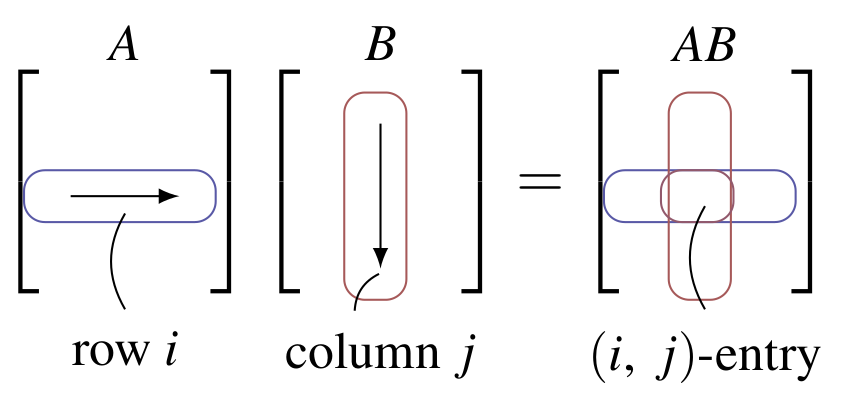
\includegraphics[scale=0.45]{DotProductRuleMatrixProduct.png}
\end{center}

\begin{example}
If $A = \begin{bmatrix} 1 & 1 & 0 \\ 0 & 1 & -1 \\ -1 & 0 & 1 \end{bmatrix}$ and $B = \begin{bmatrix} 3 & 0 \\ -2 & 1 \\ 0 & 6 \end{bmatrix}$, find $AB$.
\end{example}

\begin{solution}

\end{solution}

\vfill 

\underline{\textbf{Compatibility Rule:}} The product of matrices $A$ and $B$ is only defined when the number of columns of $A$ is equal to the number of rows of $B$.

\newpage 

\begin{example}
(a) Compute the $(2, 4)$-entry of $AB$ if
	\[
		A = \begin{bmatrix} 3 & -1 & 2 \\ 0 & 1 & 4 \end{bmatrix} \quad \text{ and } \quad B = \begin{bmatrix} 2 & 1 & 6 & 0 \\ 0 & 2 & 3 & 4 \\ -1 & 0 & 5 & 8 \end{bmatrix} .
	\]
(b) Is $BA$ well defined?
\end{example}

\begin{solution}

\end{solution}

\newpage 

\begin{example}
Let $A = \begin{bmatrix} 6 & 9 \\ -4 & -6 \end{bmatrix}$ and $B = \begin{bmatrix} 1 & 2 \\ -1 & 0 \end{bmatrix}$. Compute $A^2$, $AB$, $BA$, $(AB)^\top$ and $B^\top A^\top$. 
\end{example}

\begin{solution}

\end{solution}

\vfill 

\underline{Note:} In general, $AB \neq BA$. If $AB = BA$, then we say that $A$ and $B$ \textbf{commute}.

\newpage 

\begin{theorem}
Let $a$ be a real number, and $A, B, C$ are matrices of sizes such that the indicated matrix products are defined. Then:
	\begin{enumerate}[label=\arabic*)]
		\item $IA = A$ and $AI = A$, where $I$ denotes the identity matrix of proper size.
		\item $A (BC) = (AB) C$.
		\item $A (B + C) = AB + AC$.
		\item $(B + C) A = BA + CA$.
		\item $a (AB) = (aA)B = A (aB)$.
		\item $(AB)^{\top} = B^\top A^\top$.
	\end{enumerate}
\end{theorem}

\begin{proof}
\begin{enumerate}
	\item[1)] Assume that $A = [\mathbf{a}_1 \, \, \mathbf{a}_2 \,\, \cdots \,\, \mathbf{a}_n ]$ is of dimension $m \times n$ and $I$ is the $m \times m$ identity matrix. Then
		\begin{align*}
			IA &= [I \mathbf{a}_1 \,\, I \mathbf{a}_2 \,\, \cdots \,\, I \mathbf{a}_k ] \\ 
			&= [\mathbf{a}_1 \,\, \mathbf{a}_2 \, \, \cdots \,\, \mathbf{a}_k ]
		\end{align*}
	where we used that $I \mathbf{x} = \mathbf{x}$ from Example 4 in Section 2.2.
	\item[2)] If we write $A$ in terms of its columns:
		\begin{align*}
		(B + C) A &= [ (B + C) \mathbf{a}_1 \,\,  \cdots \,\, (B + C) \mathbf{a}_n ] \\ 
		&= [ B \mathbf{a}_1 + C \mathbf{a}_1 \,\, \cdots \,\, B \mathbf{a}_n + C \mathbf{a}_n ] \\ 
		&= [B \mathbf{a}_1 \,\, \cdots \,\, B \mathbf{a}_n ] + [C \mathbf{a}_1 \,\, \cdots \,\, C\mathbf{a}_n ] \\ 
		&= BA + CA . \tag*{$\square$}
		\end{align*}
\end{enumerate}
\end{proof}

\newpage 

\begin{example}
Simplify the following expression:
	\[
		A(3B - C) + (A - 2B)C + 2B (C + 2A)
	\]
where $A$, $B$, $C$ represent matrices.
\end{example}

\begin{solution}

\end{solution}

\newpage 

\begin{example}
Show that $AB = BA$ if and only if $(A - B) (A + B) = A^2 - B^2$.
\end{example}

\begin{solution}

\end{solution}

\newpage 

\section{Block Multiplication}

\begin{definition}
A matrix is said to be \textbf{partitioned into blocks} if the entries of the matrix are themselves matrices.
\end{definition}

\begin{example}
Writing $A = [ \mathbf{a}_1 \,\, \mathbf{a}_2 \,\, \cdots \,\, \mathbf{a}_n]$ in terms of its columns.
\end{example}

\subsubsection{Matrix Product with Blocks}
\begin{example}
(a) Find a ``nice'' partition into blocks for the following matrices
\[
	A = \begin{bmatrix} 
	1 & 0 & 0 & 0 & 0 \\ 0 & 1 & 0 & 0 & 0 \\ 2 & -1 & 4 & 2 & 1 \\ 3 & 1 & -1 & 7 & 5
	\end{bmatrix} 
	\, \, \text{ and } \, \, 
	B= \begin{bmatrix}
	4 & -2 \\ 5 & 6 \\ 7 & 3 \\ -1 & 0 \\ 1 & 6
	\end{bmatrix} .
\]
(b) Use that to compute $AB$. 
\end{example}

\begin{solution}

\end{solution}

\newpage 

\begin{example}
Obtain a formula for $A^5$ where $A = \begin{bmatrix} I & X \\ 0 & 0 \end{bmatrix}$ is a square matrix and $I$ is an identity matrix.
\end{example}

\begin{solution}

\end{solution}

\vfill 

\underline{Notes:}
	\begin{itemize}
		\item Block Multiplication is useful in theory.
		\item It is also usuful in computing products of large matrices in a computer with limited memory capacity.
	\end{itemize}

\end{document}